% !TeX root = ../thesis_main.tex

% ---------------------------------------------------
% ----- Chapters of the template
% ----- for Bachelor-, Master thesis and class papers
% ---------------------------------------------------
%  Created by C. Müller-Birn on 2012-08-17, CC-BY-SA 3.0.
%  Freie Universität Berlin, Institute of Computer Science, Human Centered Computing. 
%
\chapter{Theoretical background}
\label{chap:background}

Before discussing the design and implementation of the UI Editor, it is necessary to give a brief overview of the applied parts of HCI and the specific context, challenges and opportunities in which the UI Editor was developed.
% 

\section{Applied human-computer interaction methods}

This section concretizes the HCI aspects of this thesis and describes how and why the subject is approached from a not so common point of view.
HCI is a complex topic with a long list of available methods and even more ways to adapt them to a concrete project, so it is impossible to cover all aspects.
The UI Editor development faced challenges in integrating with an existing ecosystem and meeting technical requirements in a \gls{brownfield} project.
In my opinion, technical requirements face only limited coverage in HCI literature.
Therefore, the focus was set on them during this case study.
\\
To determine the initial functional requirements, qualitative user research methods like moderated observations (\ref{subsec:modobs}) and interviews (\ref{subsec:interview}) were chosen to be applied in an initial Design Thinking phase.
While quantitative research methods were also used to get insights during the testing phase, the decision was made against using them for this phase.
The available user base was small enough to get meaningful and representative statements only from qualitative research.
A questionnaire would either be too long or not provide enough helpful insights.
\\
Furthermore, the two concepts "SMART goals" and "three major factors of HCI" were used as foundation and guidelines during the process, which is described in chapter \ref{chap:research} in more detail.

\section{Project specific background}

In the following the functional and technical backgrounds are described to gain an understanding of the application domain.

\subsection{Functional background}

The publishing houses respectively their digital departments (in the following \textit{customer}) purchase the license for an app or website (in the following just \textit{app}, as there is not much difference besides the end medium).
Then, they can import content via multiple ways into the system, or the editors write the content directly inside the tools provided as \Gls{saas}.

\begin{figure}[h!]
  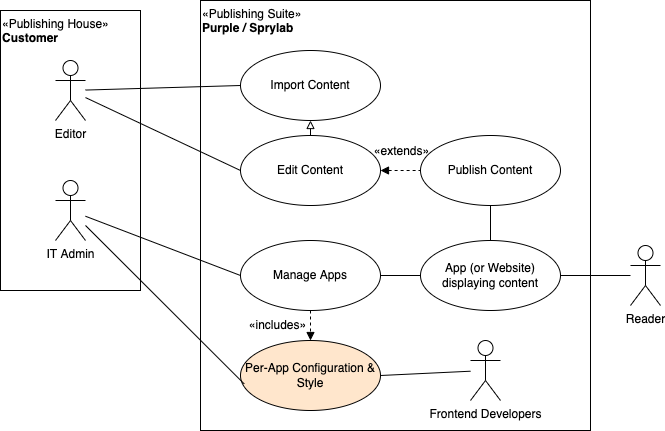
\includegraphics[width=\textwidth]{pics/purple-abstract.drawio.png}
  \caption{Use case diagram: interactions from publishers, readers and frontend developers with the system TODO: position}
  \label{fig:usecase1}
\end{figure}

The UI Editor fits into the use case "Per App configuration \& style" (see fig. \ref*{fig:usecase1}), with which mostly Frontend Developers and Project Managers from Sprylab as well as some external customer's IT Admins will interact. The goal is to lower the editing burden as much as possible, so that more of the configuration can be handed off to external customers while also improving usability for the developers of the company.

\subsection{Technical background}

The UI Editor will be implemented within the context of the proprietary web framework named \Gls{experience} which is built on top of Angular.
This framework allows complete configurability through JSON files, including routing, rendering of different components, connecting data sources, loading assets and styling the page with CSS.
These configs and assets are stored in a per-app file system called \label{def:DynamicResources} dynamic resources.
\\\\
Dynamic resources are individually managed and loaded for every app. This way, on mobile phones the end users download a native core app, which in turn just downloads the dynamic resources and executes the angular app with the configs provided from the resources.
Similar, when an end user requests a website, the backend server just looks up the dynamic resources matching this app's domain and renders the website using that config.
As a result, all customers can share the same server instance(s) in case of websites, or at least do not require extra native sourcecode changes per app.
\\
In addition, there are preview and live resources for every app, so that changes can be tested before they are released to the end users. (see fig. \ref{fig:dynres})
\begin{figure}[h!]
  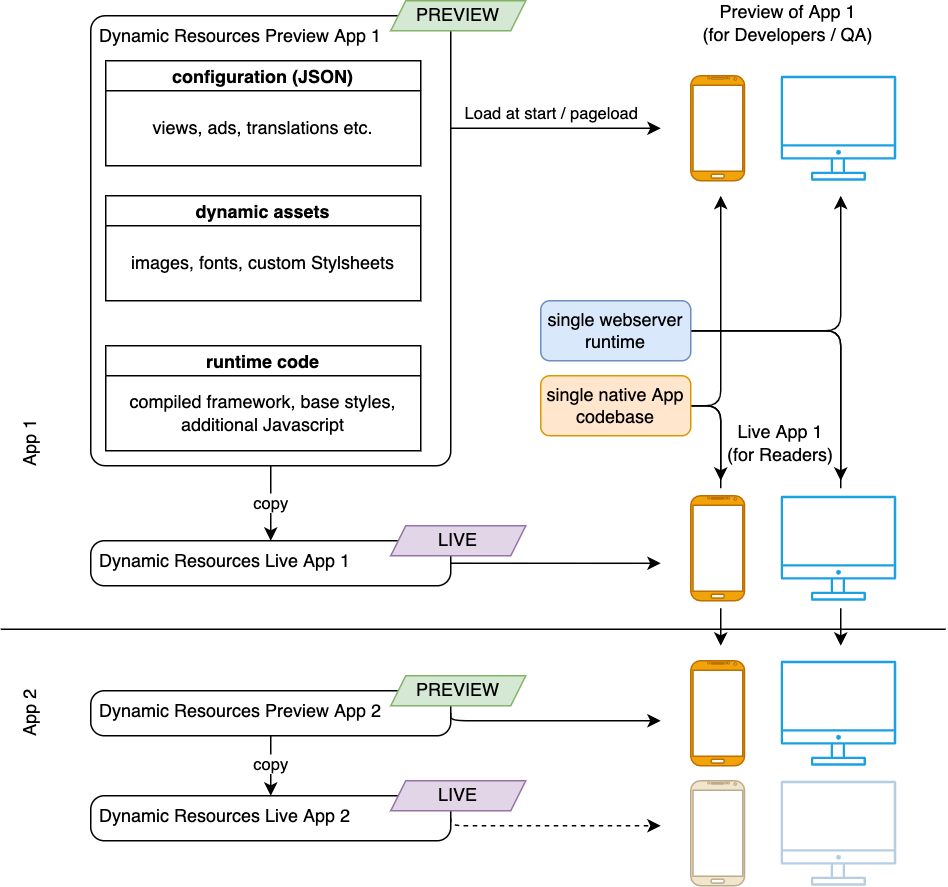
\includegraphics[width=\linewidth]{pics/experience_resources.drawio.png}
  \caption{Sprylab preview and live dynamic resources for two imaginary apps}
  \label{fig:dynres}
\end{figure}
\\
Working with large and deeply nested JSON files quickly becomes convoluted.
Manual handling of ZIP files, including modification of assets, repackaging, and the subsequent risk of introducing errors, is a labor-intensive and error-prone workflow.
\\
As a base for making editing of these configuration JSON files easier, Purple Experience generates JSON Schema files directly from the interfaces in the source code for every released version.
JSON Schema is a specification and a declarative language "that allows you to annotate and validate JSON documents." (Retrieved 11th January 2023, from \url{https://json-schema.org/}).
The use of UI elements generated from JSON Schemas allows for direct validation of user input and prevents the entry of invalid states.

At Sprylab exists a tool called "Storefront Editor", which is the predecessor for this new UI Editor.
It uses an open source software called \textit{Json Editor} (\url{https://github.com/json-editor/json-editor}), which is an implementation of the UI elements for JSON validation mentioned above.
In chapter \ref{chap:research}, the state of the JSON Editor for that use case is evaluated and the positive aspects and approaches which I reused for the new editor are generally outlined.
Furthermore, features are described which are missing, or the interview candidates noted as confusing, not working or slowing down their work.

\begin{figure}[h]
  \lstset{language=json,basicstyle=\footnotesize,numbers=left,showstringspaces=false,frame=single}
  \begin{lstlisting}
{
  "type": "view",
  "path": "/newsstand",
  "content": [
    {
      "type": "list",
      "content": {
        "type": "issue"
      },
      "dataSource": {
        "type": "issue",
        "filter": {
          "purchased": {
            "value": true
          }
        }
      }
    }
  ]
}
  \end{lstlisting}
  \caption{Simplified example of a view configuration showing purchased issues}
  \label{fig:viewexample}
\end{figure}

Figure \ref{fig:viewexample} shows a minimal example of a view configuration with which the Purple Experience could render a simple page.
The page would be accessible under the domain of the app; for example \textit{https://app1.com/newsstand} and show a list of issue components.
The data for these components is taken from the data source of type \textit{issue} which filters the published content for issues that are purchased by the current user. 
\\
In public apps, the configs are more advanced with conditionals declaring when components are rendered or filters are applied, event handlers when a user interacts with an element and many more functionalities that are modelled through the JSON Schema.


\section{Related Work}

TODO